
%% bare_jrnl_compsoc.tex
%% V1.4a
%% 2014/09/17
%% by Michael Shell
%% See:
%% http://www.michaelshell.org/
%% for current contact information.
%%
%% This is a skeleton file demonstrating the use of IEEEtran.cls
%% (requires IEEEtran.cls version 1.8a or later) with an IEEE
%% Computer Society journal paper.
%%
%% Support sites:
%% http://www.michaelshell.org/tex/ieeetran/
%% http://www.ctan.org/tex-archive/macros/latex/contrib/IEEEtran/
%% and
%% http://www.ieee.org/

%%*************************************************************************
%% Legal Notice:
%% This code is offered as-is without any warranty either expressed or
%% implied; without even the implied warranty of MERCHANTABILITY or
%% FITNESS FOR A PARTICULAR PURPOSE! 
%% User assumes all risk.
%% In no event shall IEEE or any contributor to this code be liable for
%% any damages or losses, including, but not limited to, incidental,
%% consequential, or any other damages, resulting from the use or misuse
%% of any information contained here.
%%
%% All comments are the opinions of their respective authors and are not
%% necessarily endorsed by the IEEE.
%%
%% This work is distributed under the LaTeX Project Public License (LPPL)
%% ( http://www.latex-project.org/ ) version 1.3, and may be freely used,
%% distributed and modified. A copy of the LPPL, version 1.3, is included
%% in the base LaTeX documentation of all distributions of LaTeX released
%% 2003/12/01 or later.
%% Retain all contribution notices and credits.
%% ** Modified files should be clearly indicated as such, including  **
%% ** renaming them and changing author support contact information. **
%%
%% File list of work: IEEEtran.cls, IEEEtran_HOWTO.pdf, bare_adv.tex,
%%                    bare_conf.tex, bare_jrnl.tex, bare_conf_compsoc.tex,
%%                    bare_jrnl_compsoc.tex, bare_jrnl_transmag.tex
%%*************************************************************************


% *** Authors should verify (and, if needed, correct) their LaTeX system  ***
% *** with the testflow diagnostic prior to trusting their LaTeX platform ***
% *** with production work. IEEE's font choices and paper sizes can       ***
% *** trigger bugs that do not appear when using other class files.       ***                          ***
% The testflow support page is at:
% http://www.michaelshell.org/tex/testflow/


\documentclass[10pt,conference,onecolumn,compsoc]{IEEEtran}


\usepackage{hyperref}
\usepackage{enumitem}
\setlist[itemize]{leftmargin=3 cm}
\setlist[enumerate]{leftmargin=3cm}



% *** CITATION PACKAGES ***
%
\ifCLASSOPTIONcompsoc
  % IEEE Computer Society needs nocompress option
  % requires cite.sty v4.0 or later (November 2003)
  \usepackage[nocompress]{cite}
\else
  % normal IEEE
  \usepackage{cite}
\fi
% cite.sty was written by Donald Arseneau
% V1.6 and later of IEEEtran pre-defines the format of the cite.sty package
% \cite{} output to follow that of IEEE. Loading the cite package will
% result in citation numbers being automatically sorted and properly
% "compressed/ranged". e.g., [1], [9], [2], [7], [5], [6] without using
% cite.sty will become [1], [2], [5]--[7], [9] using cite.sty. cite.sty's
% \cite will automatically add leading space, if needed. Use cite.sty's
% noadjust option (cite.sty V3.8 and later) if you want to turn this off
% such as if a citation ever needs to be enclosed in parenthesis.
% cite.sty is already installed on most LaTeX systems. Be sure and use
% version 5.0 (2009-03-20) and later if using hyperref.sty.
% The latest version can be obtained at:
% http://www.ctan.org/tex-archive/macros/latex/contrib/cite/
% The documentation is contained in the cite.sty file itself.



% *** GRAPHICS RELATED PACKAGES ***
%
\ifCLASSINFOpdf
   \usepackage[pdftex]{graphicx}
 
\else
 
\fi
% graphicx was written by David Carlisle and Sebastian Rahtz. It is
% required if you want graphics, photos, etc. graphicx.sty is already
% installed on most LaTeX systems. The latest version and documentation
% can be obtained at: 
% http://www.ctan.org/tex-archive/macros/latex/required/graphics/
% Another good source of documentation is "Using Imported Graphics in
% LaTeX2e" by Keith Reckdahl which can be found at:
% http://www.ctan.org/tex-archive/info/epslatex/
%
% latex, and pdflatex in dvi mode, support graphics in encapsulated
% postscript (.eps) format. pdflatex in pdf mode supports graphics
% in .pdf, .jpeg, .png and .mps (metapost) formats. Users should ensure
% that all non-photo figures use a vector format (.eps, .pdf, .mps) and
% not a bitmapped formats (.jpeg, .png). IEEE frowns on bitmapped formats
% which can result in "jaggedy"/blurry rendering of lines and letters as
% well as large increases in file sizes.
%
% You can find documentation about the pdfTeX application at:
% http://www.tug.org/applications/pdftex









% *** PDF, URL AND HYPERLINK PACKAGES ***
%
\usepackage{url}
% url.sty was written by Donald Arseneau. It provides better support for
% handling and breaking URLs. url.sty is already installed on most LaTeX
% systems. The latest version and documentation can be obtained at:
% http://www.ctan.org/tex-archive/macros/latex/contrib/url/
% Basically, \url{my_url_here}.




\begin{document}

\title{Coding with Octocat}
%
%

% received ..."  text while in non-compsoc journals this is reversed. Sigh.

\author{Jennifer Huestis and Trever Hall% <-this % stops a space
}

\IEEEtitleabstractindextext{%
\begin{abstract}
The project is a side scroller that draws inspiration from Google Chromes' dinosaur game easter egg. It is going to be computer science themed with Octocat running and trying to avoid "bugs and broken windows" as obstacles. The form of currency in the game is energy by caffeinated products, which can be used to buy in game upgrades. The main goal is to survive as long as possible, and you are told the total distance you traveled (given by a running counter).
\end{abstract}

}


% make the title area
\maketitle



\IEEEdisplaynontitleabstractindextext

\IEEEpeerreviewmaketitle



\section{Introduction}

This is a project that we are doing for a class. We don't expect to publish it or for it to have a large user-base, but we think it will be a fun and challenging game that is simple enough for anyone to play. It will follow the generic platformer design with the player auto running and incrementing the speed the longer you survive. The user will have to jump to try and avoid the obstacles. The player only has one life, so once they hit an obstacle they die.
\\

Challenges we foresee are getting the screen to scroll and making sure everything is timed correctly so that the pixel art actually looks like it is moving. If it is not as challenging as we foresee, then we also have some stretch goals that we think would be nice to add to the game. Those would be things like adding more items into the game and having long-term high scores.



\subsection{Background}
If not familiar with the concept of a platformer, it is a two dimensional game with a player that can move within that plane. Examples of games like that include the original Mario games, Flappy Birds, Terraria, Donkey Kong and many more! These games of our childhood have inspired us to create one of our very own.


\subsection{Challenges}
There are many challenges to cresting a video game in WPF, but ones that stand out to us are: scrolling, timing, and pixel art.

\subsubsection{Scrolling} The screen needs to scroll to the right. That is going to require auto generation of the screen from the right and deletion from the left to give the user the illusion of movement. 

\subsubsection{Timing}There are many elements that rely on a system for keeping track of time. The obvious one is the user needs to know how long they survived. Other than that though, enemy and player velocity depend on the amount of time passed (in this instance pixels per second).

\subsubsection{Pixel Art}All graphics are going to be complicated since its on WPF, and we must implement a system that consistently updates the window so that you can see the graphics move. Not only do we need to time movement, but we also need to change the art with every update so that it looks like characters are moving (walking, running, flying, etc).



\section{Scope}
The game begins with Octocat auto running toward the right after a user hits "start". When Octocat is running randomized obstacles (broken windows and bugs) will generate from the right of the window; the player will have to avoid them by jumping or ducking. The further you survive (distance is displayed on the screen and counting as you play) the faster the Octocat will run. When you die it will display the distance that you traveled as well as items collected on that round. The user can use energy from caffeinated items they pick up to buy upgrades (minimally one upgrade). The requirements seem simple at first, but are difficult to fulfill.


\subsection{Stretch Goals}
There are a lot of additions we would like to add to the game, but two that we believe would add the most to the user experience are long-term high scores and adding more power ups and other useful items into the game.

\subsubsection{Stored High Scores}
We want to keep a record of the top ten scores and allow the user to enter a name to associate with it (just three letters like the retro games in arcades). This should be accessible from a button on the menu. The goal is to make it keep track even if you close the game and re-open it.

\subsubsection{More Items} We want to add more items to buy. Things that we would like to include are an invincibility power-up where Octocat will start riding a flying rainbow cat avoiding all obstacles, a companion (it just follows the player around), and a variety of colors for Octocat.

\subsection{Requirements}
To make the game functional and provide each user with a good experience, it will have to follow the requirements we gathered below:

\subsubsection{Functional}
\begin{itemize}
\item User is able to toggle music volume on and off.
\item Users is able to toggle sound effects on and off.
\item User is able to purchase items.
\item User is able to record three character name with high scores.
\item User is able to quit the application.
\item User is able to jump and duck to avoid obstacles.
\item User is able to use inventory items during the game.
\item User's character detects collision with obstacles and items and reacts accordingly.
\end{itemize}

\subsubsection{Non-Functional}
\begin{itemize}
\item Platform -- user can only run the application on capable windows machines.
\item Usability -- There is no native support for those with disabilities that may hinder the users experience.
\item Reliability -- The program will not stop running until the user closes it.
\item Data Integrity -- The high scores will be stored locally and maintained by the game.
\item Maintainability -- Once finished the game should not need any maintenance.
\end{itemize}

\subsection{Use Cases}

A user is able to follow the steps of the use cases provided below and get the specified outcome every time.

\begin{table}[hp]
\centering
\begin{tabular}{|c|c|c|c|c|}
\hline
Use Case ID & Use Case Name & Primary Actor & Complexity & Priority \\
\hline \hline
1 & Adding a New High Score & Normal User & Med & 1\\
\hline
2 & Purchase an Item & Normal User & Med & 1\\
\hline
3 & View High Scores & Normal User & Low & 2\\
\hline
4 & Accessing Information & Normal User & Low & 2\\
\hline
5 & Start the Game & Normal User & Med & 1\\
\hline
6 & Change Octocat's Skin & Normal User & Med & 3\\
\hline
7 & Toggle Music on/off & Normal User & Low & 3\\
\hline
8 & Toggle Sound Effects on/off& Normal User & Low & 3\\
\hline
9 & Quit the Game & Normal User & Low & 2\\
\hline
10 & Avoid Obstacles & Normal User & High & 1\\
\hline
11 & Hitting Obstacles & Normal User & High & 1\\
\hline

\end{tabular}
\caption{Use case table}
\label{tab:useCaseIndex}
\end{table}


\begin{itemize}
\item[Use Case Number:] 1
\item[Use Case Name:] Adding a new high score
\item[Description:] The user has survived longer than an existing high score, or there is an empty slot in the high scores. Thus, the user is prompted to add there user three letter name to be displayed with the score.\end{itemize}

Steps to add name to go the score:

\begin{enumerate}
\item User qualifies and is prompted by the game to add a name.
\item User types in 3 letters.
\item User clicks save out beside the text field
\item[Termination Outcome:] High score table is updated and displayed.\\
\end{enumerate}

\begin{itemize}
\item[Use Case Number:] 2
\item[Use Case Name:] Purchasing an Item
\item[Description:] The user wants to purchase and item.
\item[Invariants:] The user has sufficient funds to purchase the item selected.
\end{itemize}

Steps to buy an item from the store:

\begin{enumerate}
\item User navigates to the "store" page.
\item User locates item.
\item User clicks the "Buy" button bellow the item wanted.
\item[Termination Outcome:] The price is subtracted from the users currency, and one instance if the 
item is added to the users inventory.\\
\end{enumerate}

\begin{itemize}
\item[Use Case Number:] 3
\item[Use Case Name:] Viewing High Scores
\item[Description:] The user wants to view the high scores.
\end{itemize}

Steps to view the high scores:

\begin{enumerate}
\item User navigates to the main menu.
\item User left clicks the "High Scores" button.
\item[Termination Outcome:] Screen displays high scores, and user can click the back button to return to the menu.\\
\end{enumerate}

\begin{itemize}
\item[Use Case Number:] 4
\item[Use Case Name:] Accessing Information
\item[Description:] The user wants to access background information and controls.
\end{itemize}

Steps to access information:

\begin{enumerate}
\item User navigates to the main menu.
\item User left clicks the information icon.
\item[Termination Outcome:] Moves to screen displaying the information, and user can click the back button to return to the menu.\\
\end{enumerate}

\begin{itemize}
\item[Use Case Number:] 5
\item[Use Case Name:] Start the Game.
\item[Description:] The user wants to start the game.
\item[Precondition:] User is at the start menu.
\end{itemize}

Steps to start the game:

\begin{enumerate}
\item User left clicks the "Start" button.
\item[Termination Outcome:] The game will begin and Octocat starts auto-running.\\
\end{enumerate}

\begin{itemize}
\item[Use Case Number:] 6
\item[Use Case Name:] Change Octocat's Skin
\item[Description:] The user wants to change the color of Octocat.
\item[Precondition:] User is at the start menu.
\end{itemize}

Steps to change Octocat's skin:

\begin{enumerate}
\item User left clicks the Octocat icon.
\item User selects the desired color.
\item[Termination Outcome:] The color of Octocat icon and player is updated.\\
\end{enumerate}

\begin{itemize}
\item[Use Case Number:] 7
\item[Use Case Name:] Toggle Music on/off
\item[Description:] The user want to turn the music on or off.
\item[Precondition:] User is at the start menu.
\end{itemize}

Steps to toggle the music:

\begin{enumerate}
\item User left-clicks the music icon.
\item[Termination Outcome:] The music toggles on or off.\\
\end{enumerate}

\begin{itemize}
\item[Use Case Number:] 8
\item[Use Case Name:] Toggle Sound Effects on/off
\item[Description:] The user want to turn the sound effects  on or off.
\item[Precondition:] User is at the start menu.
\end{itemize}

Steps to toggle the sound effects:

\begin{enumerate}
\item User left-clicks the sound effects icon.
\item[Termination Outcome:] The sound effects toggles on or off.\\
\end{enumerate}

\begin{itemize}
\item[Use Case Number:] 9
\item[Use Case Name:] Quit the Game
\item[Description:] The user wants to quit the game.
\item[Precondition:] User is at the start menu.
\end{itemize}

Steps to view quit the game:

\begin{enumerate}
\item User left clicks the quit icon.
\item[Termination Outcome:] The program will stop running.\\
\end{enumerate}

\begin{itemize}
\item[Use Case Number:] 10
\item[Use Case Name:] Avoid Obstacles
\item[Description:] The user wants to avoid obstacles.
\item[Precondition:] User has started the game, by clicking the start button.
\end{itemize}

Steps to avoid obstacles:

\begin{enumerate}
\item User clicks the up(jump) or down(duck) arrow to avoid an approaching obstacle.
\item[Termination Outcome:] The user does not hit the obstacle and the game continues.\\
\end{enumerate}

\begin{itemize}
\item[Use Case Number:] 11
\item[Use Case Name:] Hitting Obstacles
\item[Description:] The user fails to avoid an obstacle.
\item[Precondition:] User has started the game, by clicking the start button.
\end{itemize}

Steps to hit an obstacle:

\begin{enumerate}
\item The user does not use the arrow keys to jump(up) or duck(down) at the right time.
\item[Termination Outcome:]The user hits the obstacle and dies (unless saved by an item).
\end{enumerate}


\begin{figure}[h!]
\centering
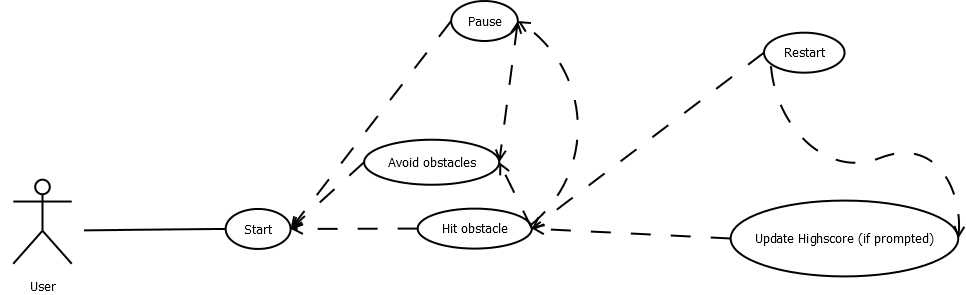
\includegraphics[scale=.4]{Start.png}
\caption{Use case to start the game and all of the use cases that it interacts with.}
\label{Start}

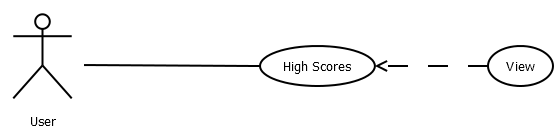
\includegraphics[scale=.5]{HighScores.png}
\caption{Use case for viewing high scores.}
\label{Scores}
\end{figure}

\begin{figure}[h!]
\centering
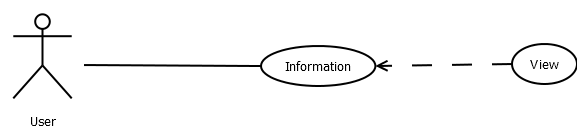
\includegraphics[scale=.5]{Information.png}
\caption{Use case to view information.}
\label{Info}

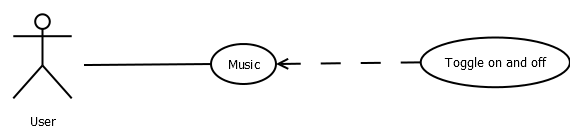
\includegraphics[scale=.5]{Music.png}
\caption{Use case to toggle music.}
\label{Music}

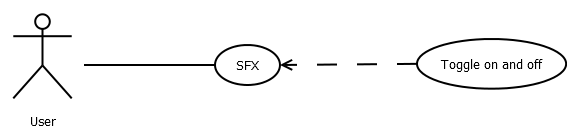
\includegraphics[scale=.5]{SFX.png}
\caption{Use case to toggle sound effects.}
\label{SFX}

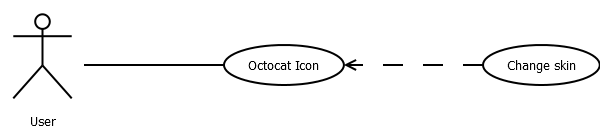
\includegraphics[scale=.5]{Octocat_Icon.png}
\caption{Use case to change Octocat's skin.}
\label{Skin}

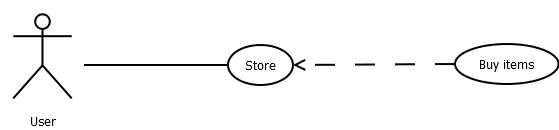
\includegraphics[scale=.5]{Store.png}
\caption{Use case to buy items from the store.}
\label{Store}

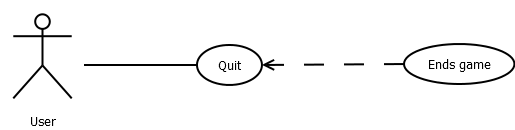
\includegraphics[scale=.5]{Quit.png}
\caption{Use case to quit the game.}
\label{Quit}
\end{figure}


\clearpage

\subsection{Interface Mockups}
The mockups below are a rough draft for the design of the games interfaces. It is not exactly what the final project will look like, but does introduce what screens should be available and how the user will interact with them.


\begin{figure}[!ht]
\centering
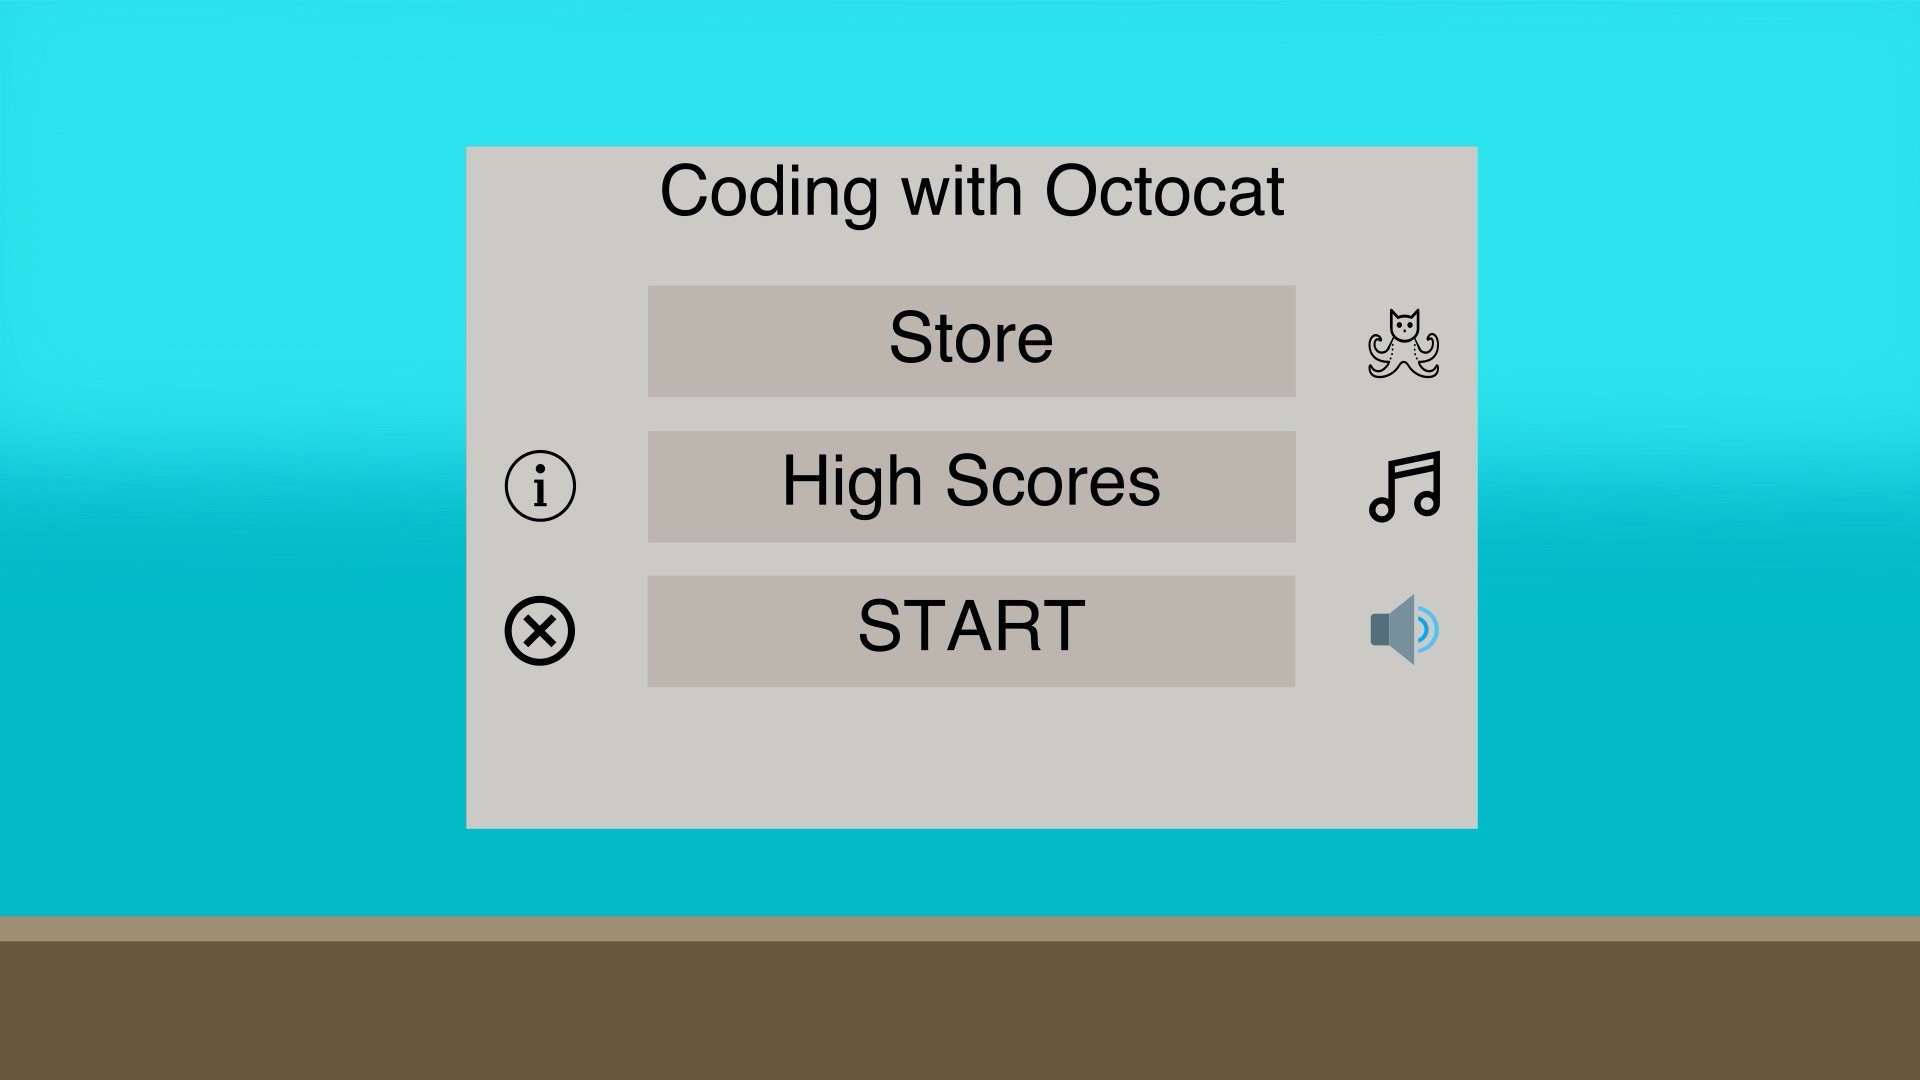
\includegraphics[scale=.2]{MockupStartScreen.jpeg}
\caption{The start screen and menu where you can interact with the following use cases: start, view high scores, store, change skin, toggle music, toggle sound effects, view information, and quit.}

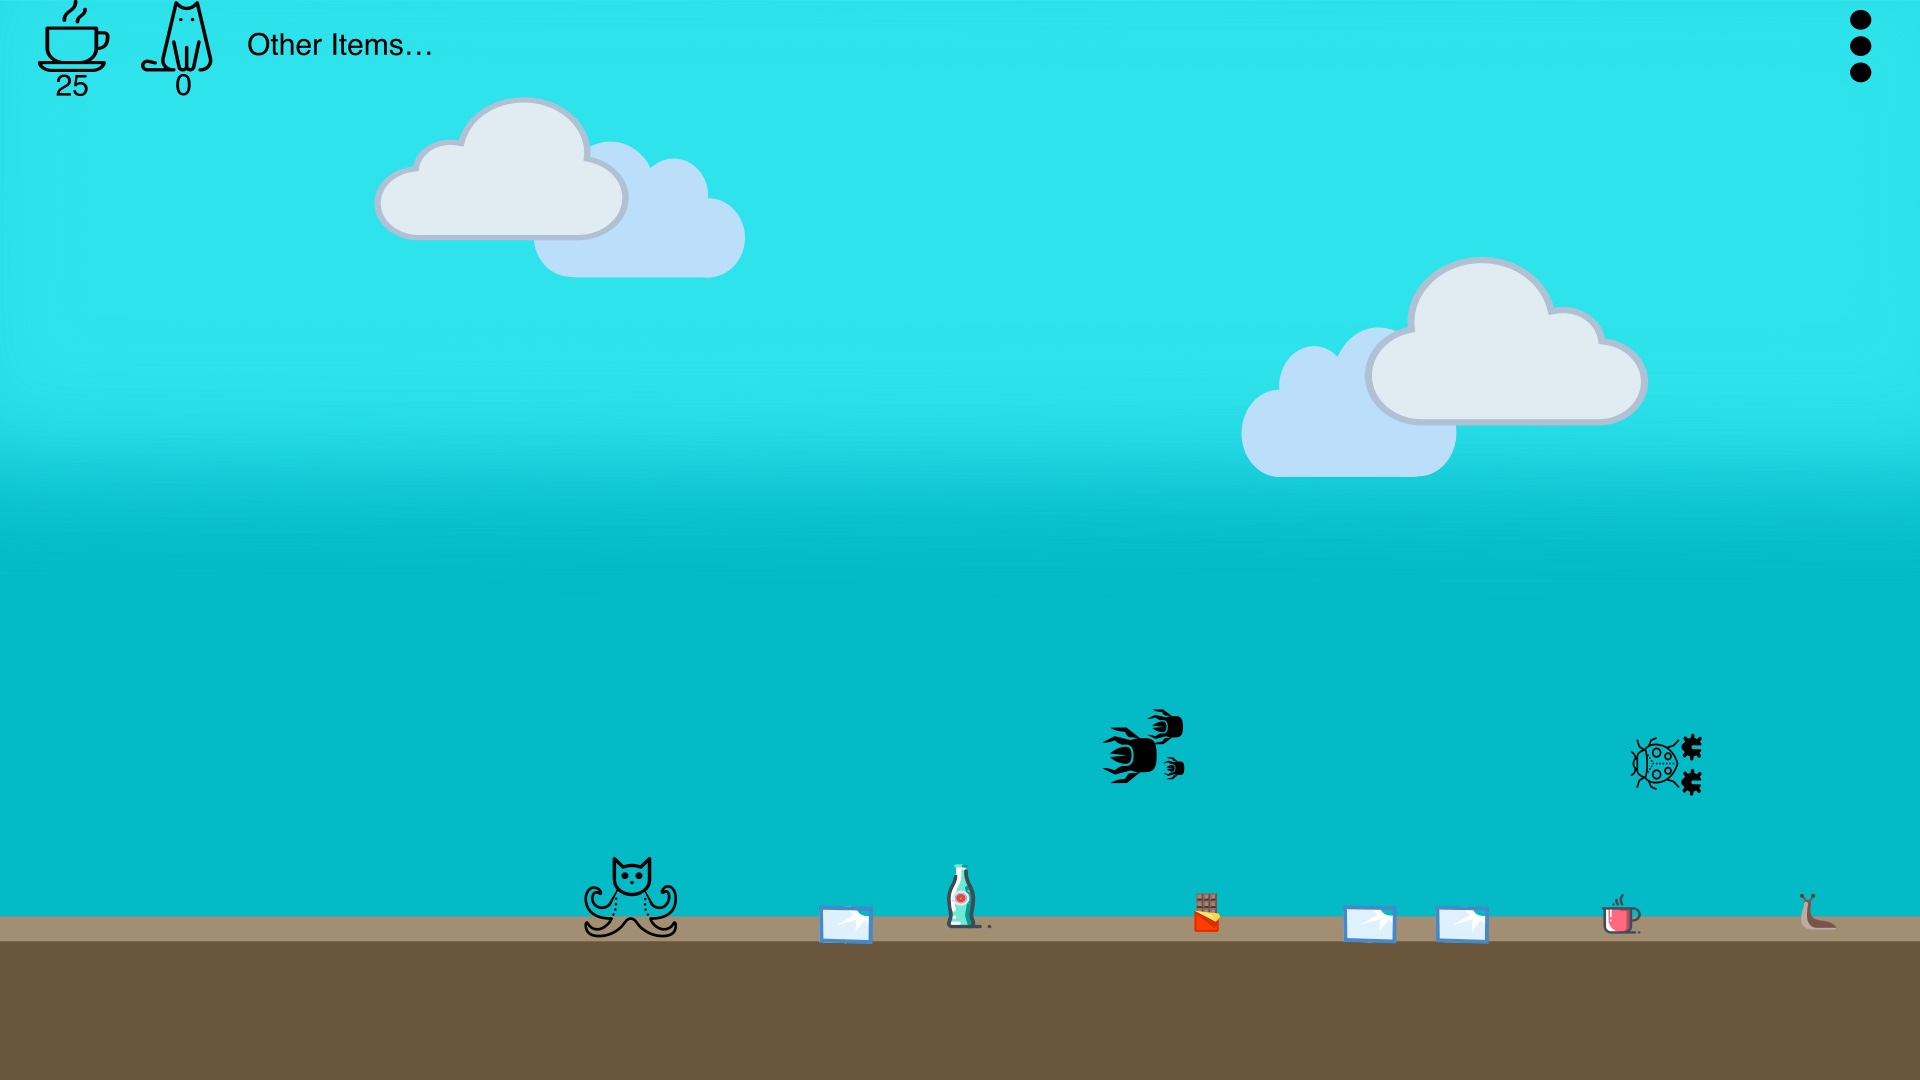
\includegraphics[scale=.2]{MockupIngame.jpeg}
\caption{The screen where the user is in the game trying to avoid obstacles. }
\end{figure}

\begin{figure}[!ht]
\centering
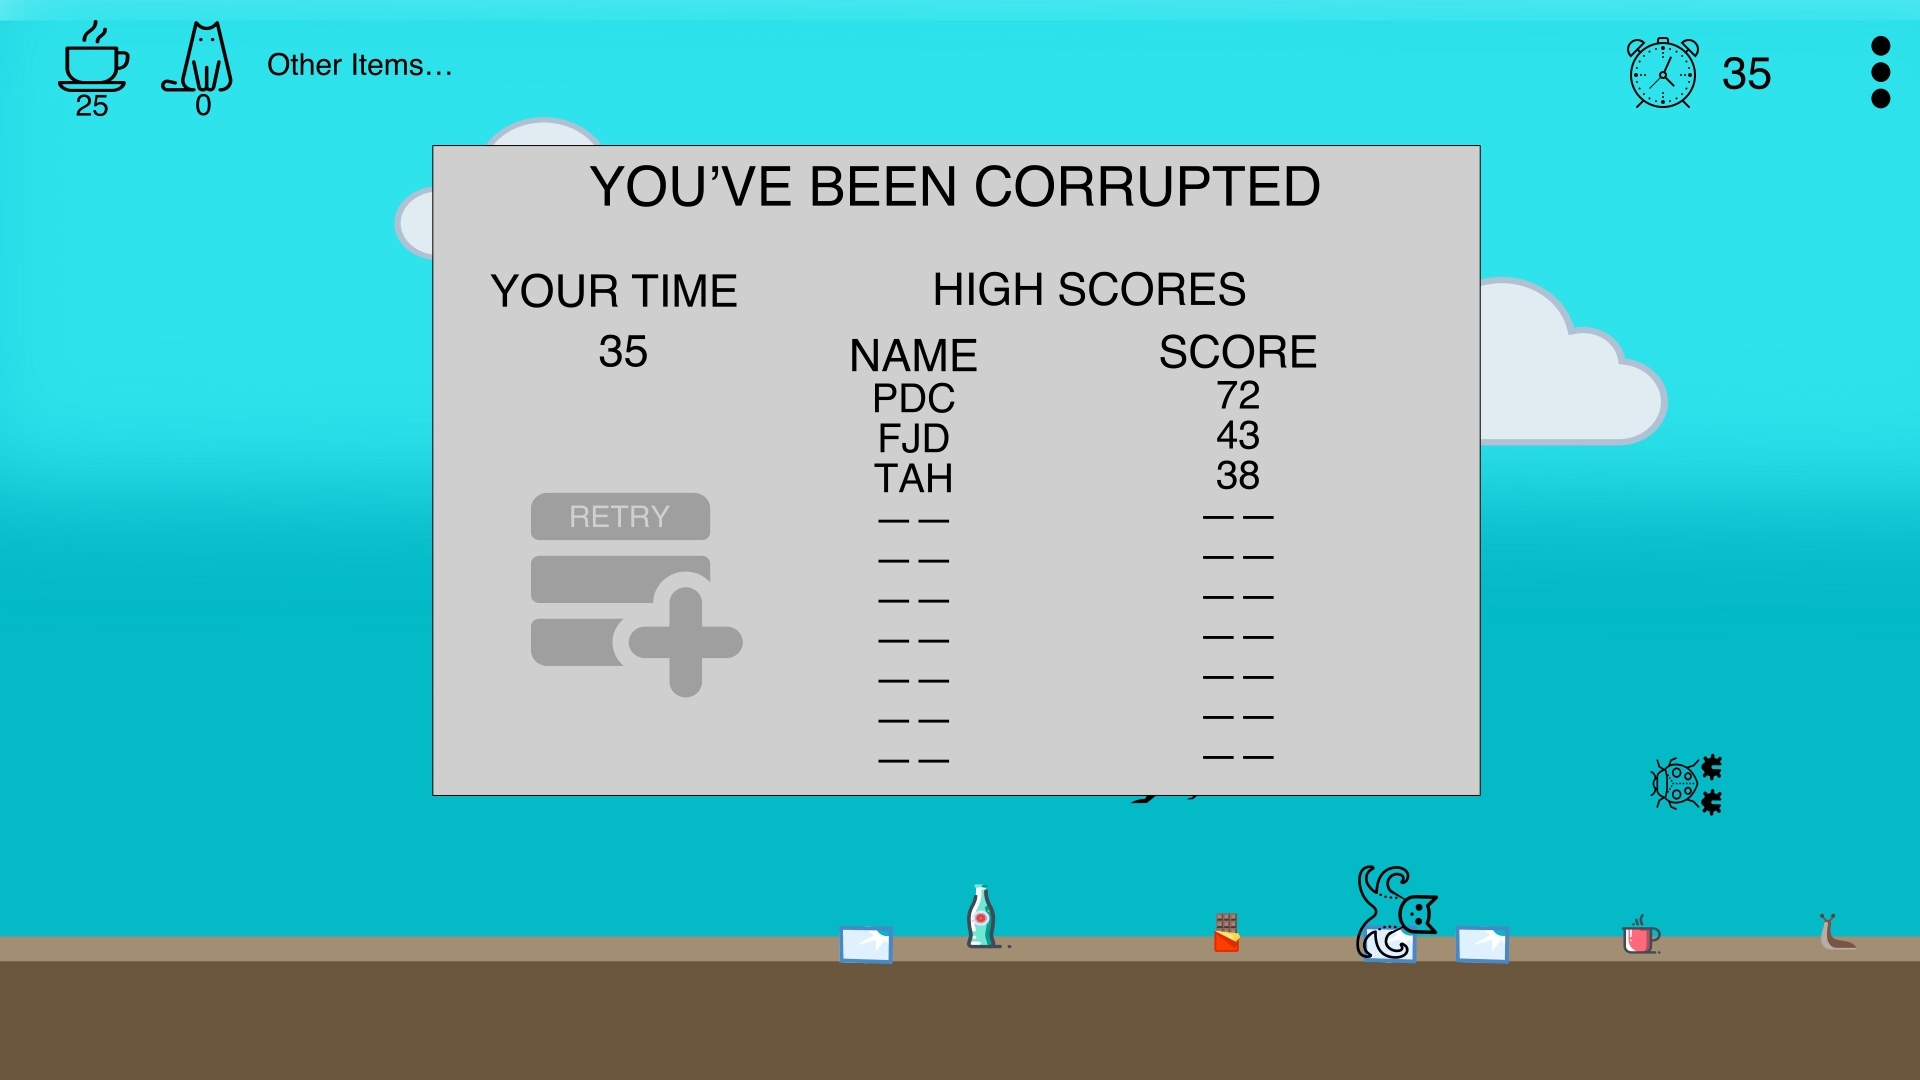
\includegraphics[scale=.2]{MockupEndgame.jpeg}
\caption{The screen where the user sees stats after they hit an obstacle and can restart.}

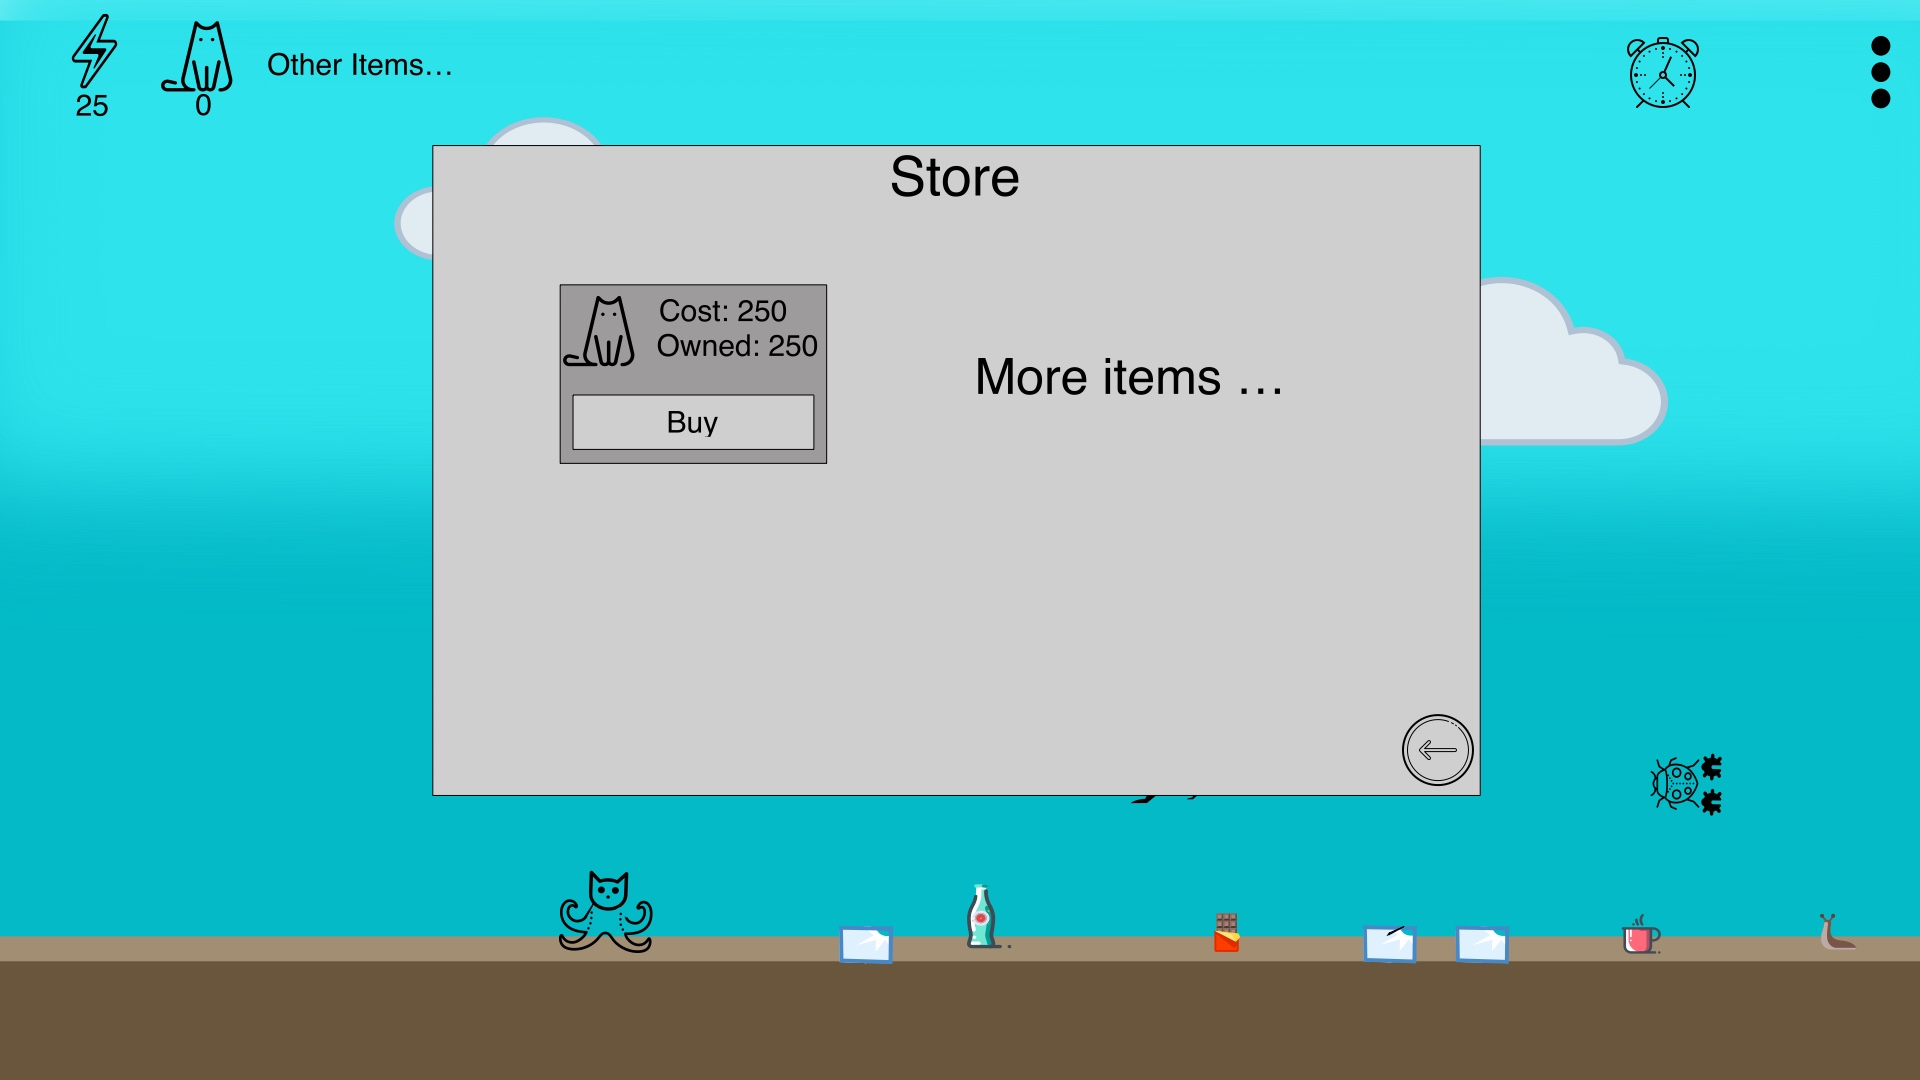
\includegraphics[scale=.2]{MockupStore.jpeg}
\caption{The screen where the user can buy items and upgrades.}

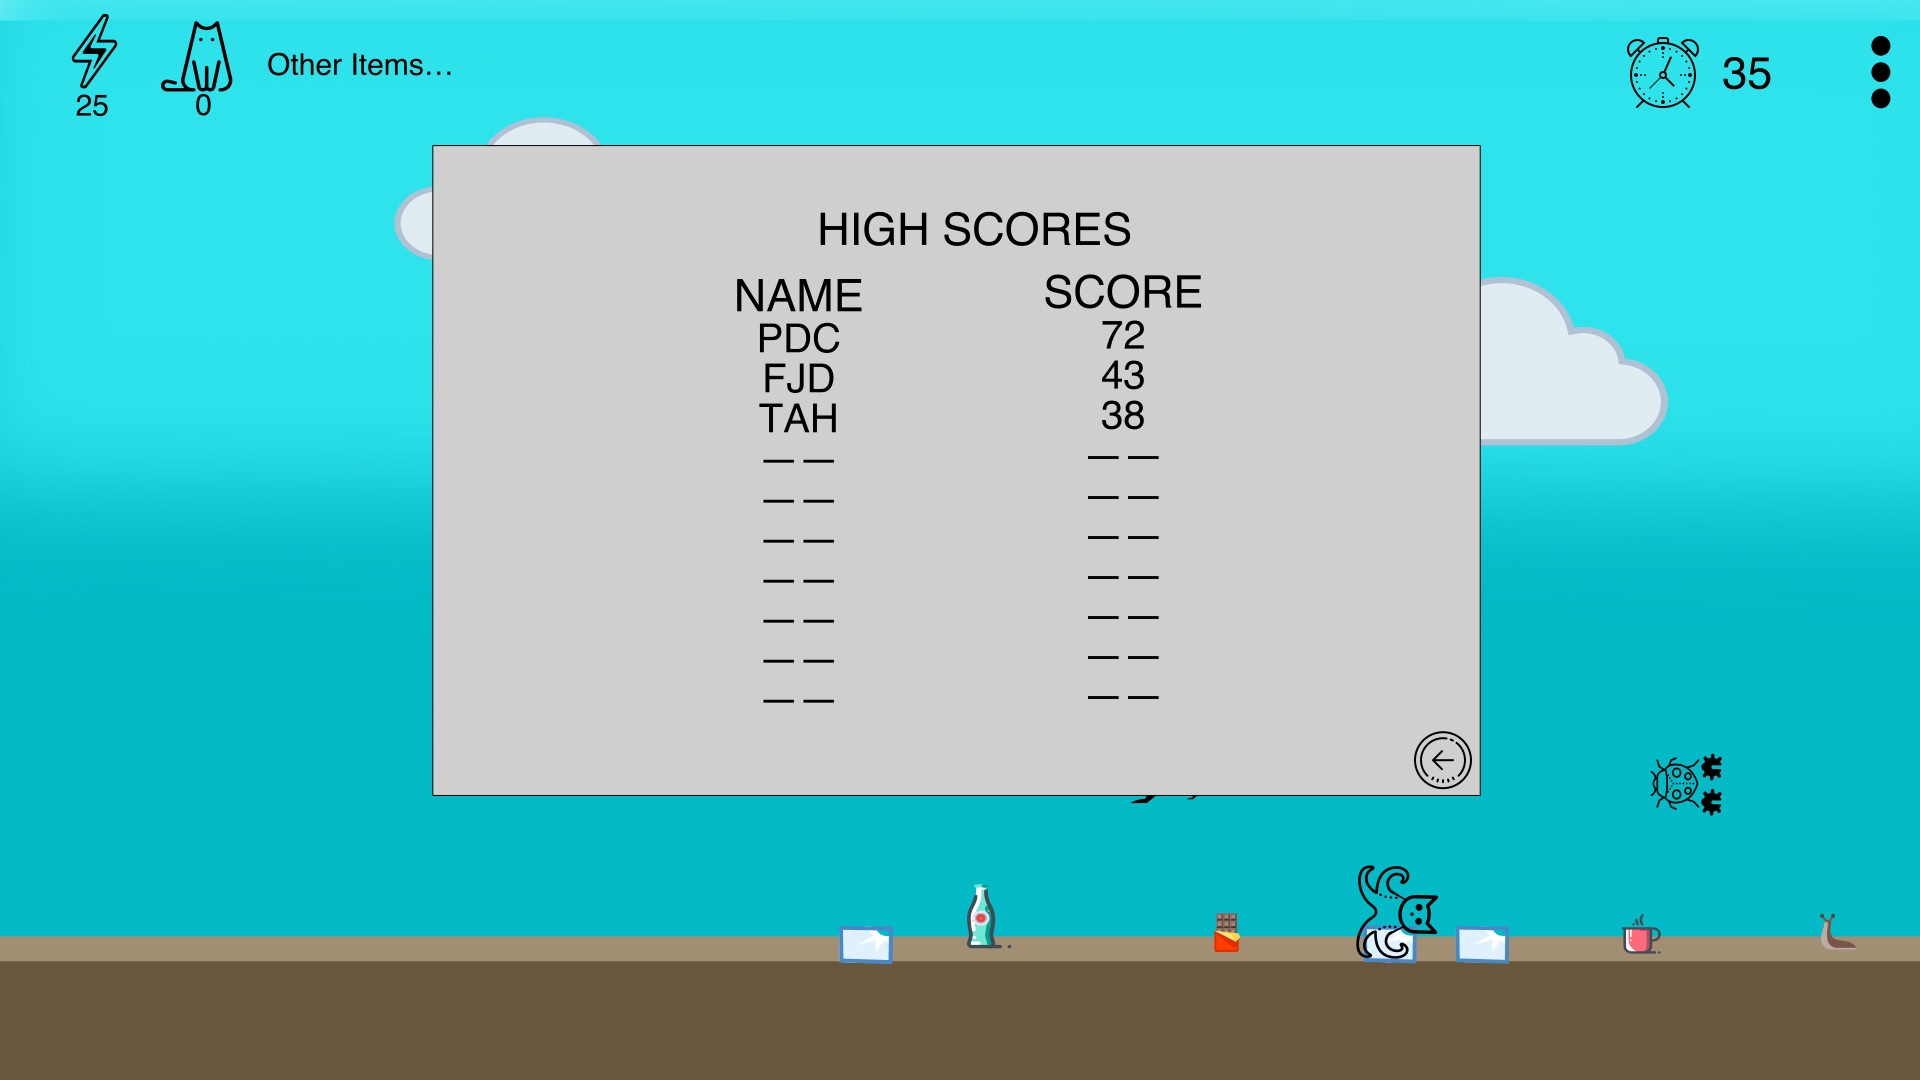
\includegraphics[scale=.2]{MockupHighscores.jpeg}
\caption{The screen where the user can view the high scores.}

\end{figure}

\clearpage

\section{Project Timeline}
To make sure we can keep track of what needs to be done when for the project, we have generated a timeline shown in figure 14 that outlines important tasks and when to accomplish them within 30 days. Some tasks are optional, so those have been placed at the end—even though we may not get to them.

\begin{figure}[!ht]
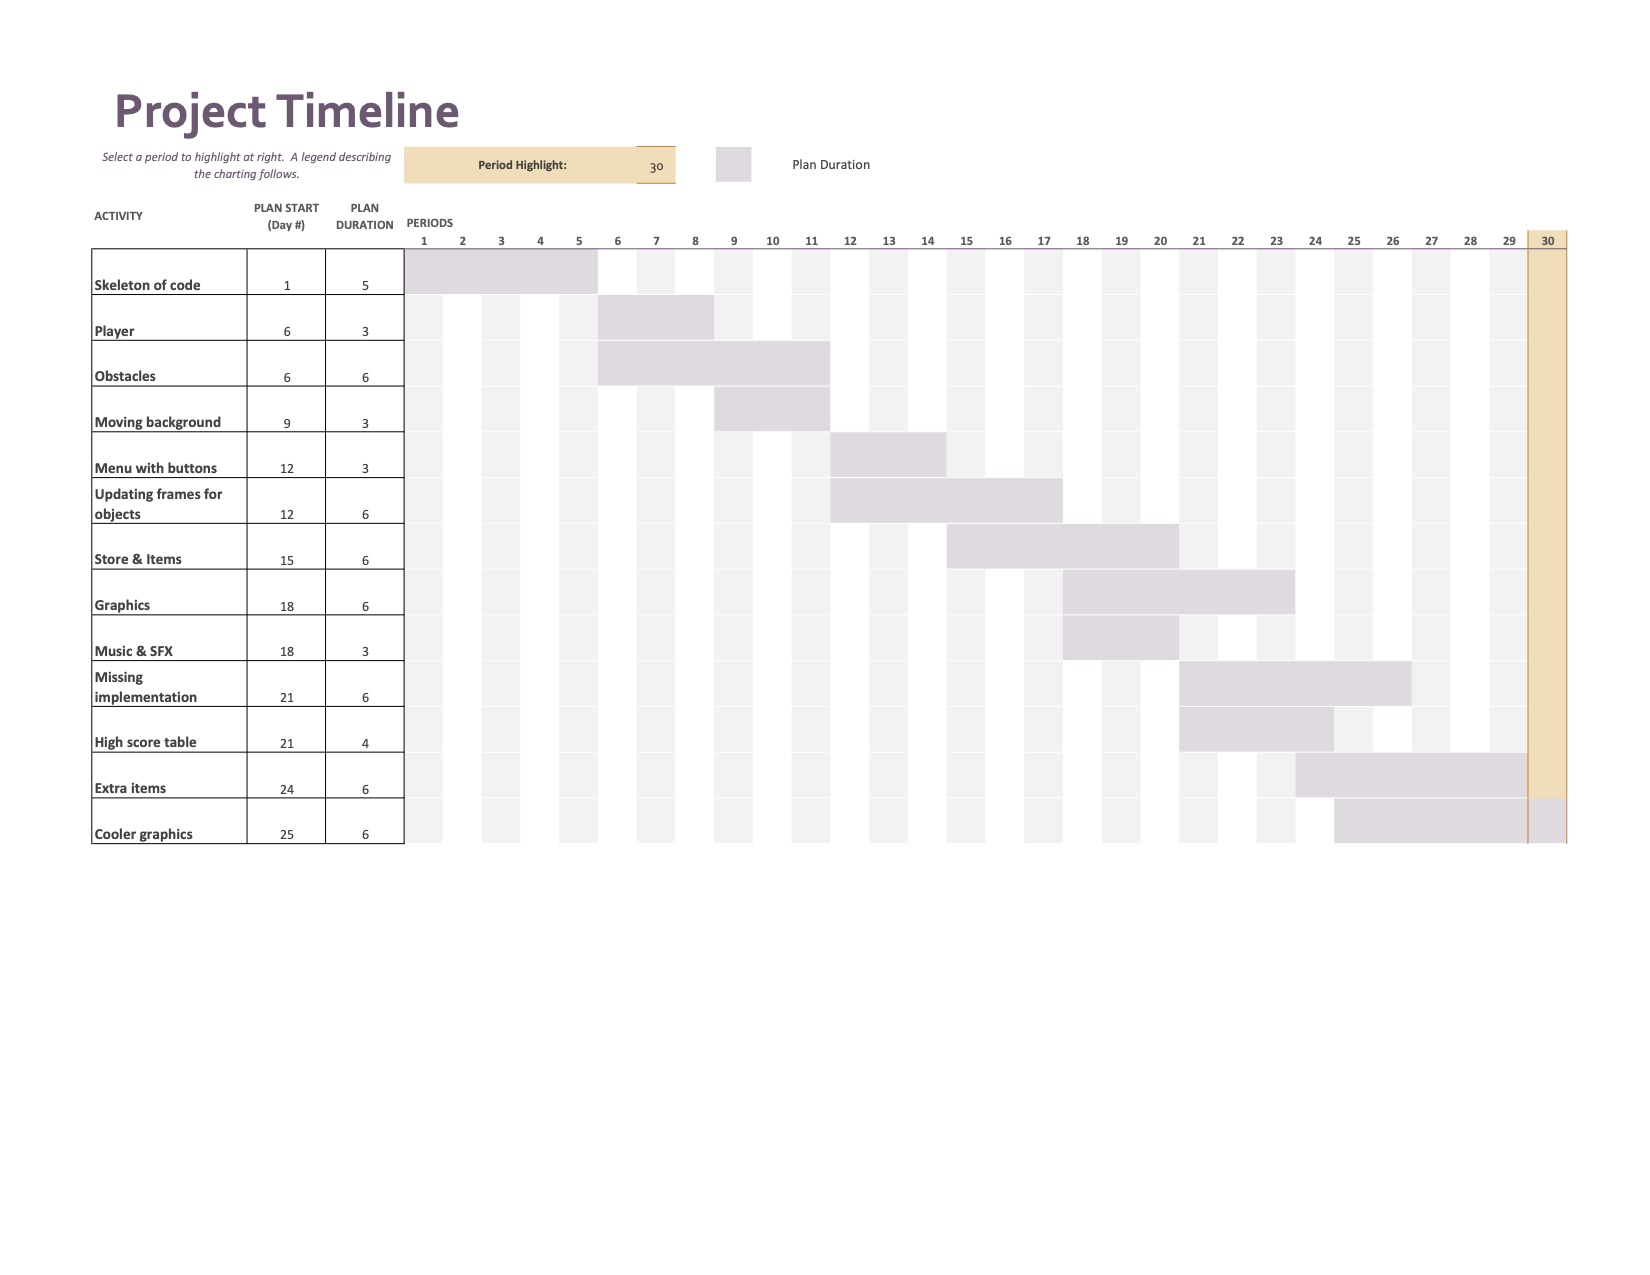
\includegraphics[scale=.3]{Timeline.jpeg}
\caption{Timeline for the last 30 days of the project.}
\end{figure}

\section{Project Structure}
Our project is outlined in a UML that breaks Coding with Octocat down into classes, and it includes three design patterns that group classes together for certain tasks.

\subsection{UML Outline}
The UML outline shown below in figure 15 shows the structure of our program separated into classes that work together to make Coding with Octocat run. Some classes are grouped into design patterns; while, other classes do not need that functionality.

\clearpage

\begin{figure}[!ht]
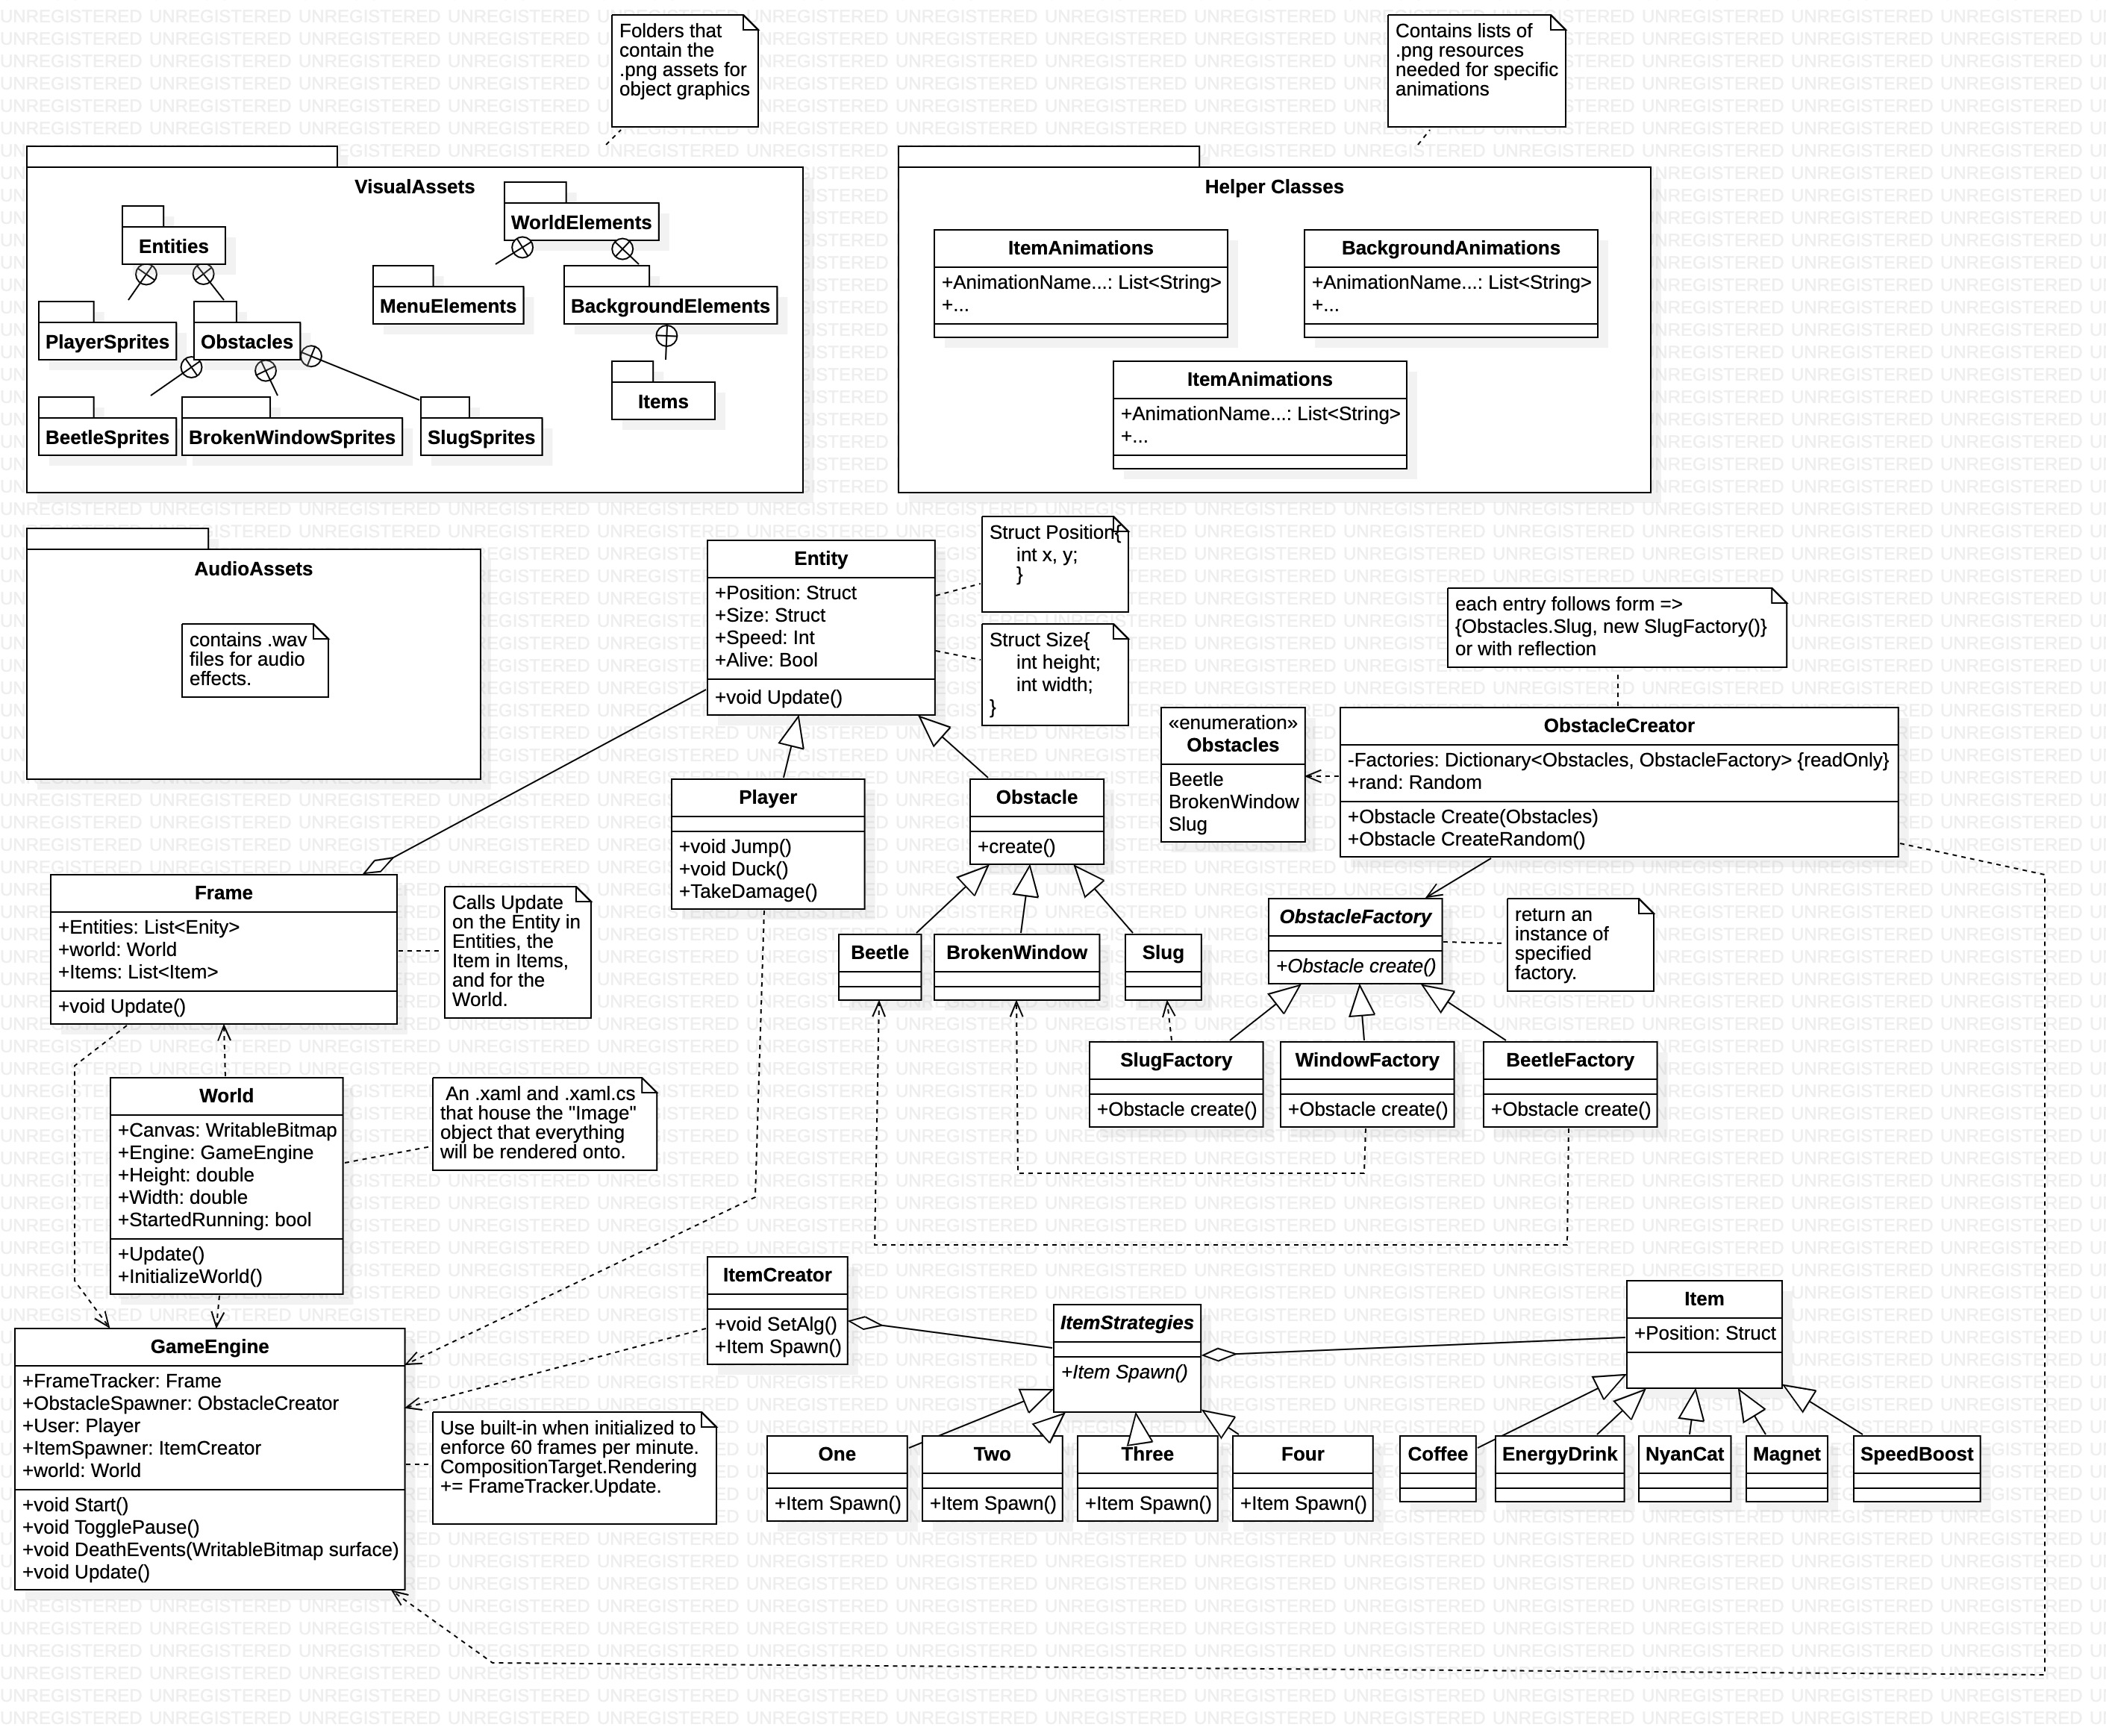
\includegraphics[scale=.18]{UML.jpg}
\caption{UML of the project.}
\end{figure}

\subsection{Design Patterns Used}
To make Coding with Octocat functional, we are using three design patterns discussed in CSCI 352, factory method, strategy, and observer. Factory method is for generating obstacles, and strategy pattern adjusts the item appearance rate based on the distance the player has traversed. Then, there is the observer pattern that is used to keep track of the frames, and tells the player, all obstacles, and all world objects to update position.

% that's all folks
\end{document}


